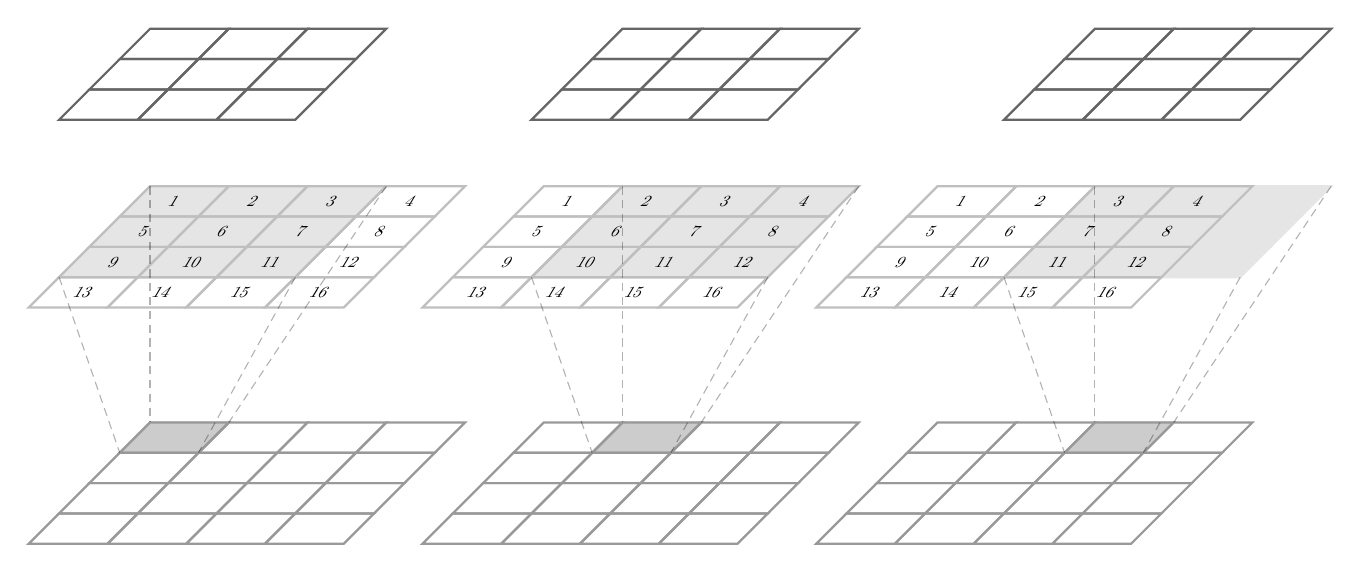
\begin{tikzpicture}
  \pgfmathsetmacro{\sep}{2.0}
  \pgfmathsetmacro{\outsep}{3.0}
  \foreach \m [count=\d] in {0,5,10} {
    \pgfmathsetmacro{\end}{\m+2}
    \pgfmathsetmacro{\END}{\m+3}

    % shadow casted by the filter
    \pgfmathsetmacro{\start}{\m + \d - 1}
    \pgfmathsetmacro{\end}{\m + 2 + \d - 1}
    \foreach \x in {\start,...,\end} { %
      \foreach \z in {0,...,2} { %
        \filldraw[thick, color=black!10] 
        (\x, 0, \z) -- 
        (\x, 0, \z - 1) -- 
        (\x + 1, 0, \z - 1) -- 
        (\x + 1, 0, \z) -- cycle;
      } %
    } %

    % input grid
    \foreach \x [count=\c] in {\m,...,\END} { %
      \foreach \z [count=\r] in {0,...,3} { %
        \draw[thick, color=black!25] 
        (\x, 0, \z) -- 
        (\x, 0, \z - 1) -- 
        (\x + 1, 0, \z - 1) -- 
        (\x + 1, 0, \z) -- cycle;

        \pgfmathtruncatemacro{\index}{\r*4 + \c - 4}
        \path (\x + 0.5, 0, \z) -- (\x + 0.5, 0, \z - 1) node[midway, 
        anchor=center, xslant=0.6, font=\footnotesize, scale=0.7]
        {$\alphalph{\index}$};
      } %
    } %

    % filter
    \pgfmathsetmacro{\start}{\m + \d - 1}
    \pgfmathsetmacro{\end}{\m + 2 + \d - 1}
    \foreach \x [count=\c] in {\start,...,\end} { %
      \foreach \z [count=\r] in {0,...,2} { %
        \draw[thick, color=black!60] (\x, \sep, \z) -- (\x, \sep, \z - 1) --
        (\x + 1, \sep, \z - 1) -- 
        (\x + 1, \sep, \z) -- cycle;
      } %
    } %

    % output convolution cell
    \filldraw[thick, color=black!20] 
    (\start, -\outsep, 0) -- 
    (\start, -\outsep, -1) -- 
    (\start + 1, -\outsep, -1) -- 
    (\start + 1, -\outsep, 0) -- cycle;
    % \path (\start + 0.5, -\outsep, 0) -- (\start + 0.5, -\outsep, -1) node[midway, 
    % anchor=center, xslant=0.6]
    % {$*$};

    % output grid
    \foreach \x [count=\c] in {\m,...,\END} { %
      \foreach \z [count=\r] in {0,...,3} { %
        \draw[thick, color=black!40] 
        (\x, -\outsep, \z) -- 
        (\x, -\outsep, \z - 1) -- 
        (\x + 1, -\outsep, \z - 1) -- 
        (\x + 1, -\outsep, \z) -- cycle;
      } %
    } %

    % connection between input and output
    \draw [densely dashed, opacity=0.3] (\start, 0, 2) -- (\start, -\outsep, 0);
    \draw [densely dashed, opacity=0.3] (\start, 0, -1) -- (\start, -\outsep, -1);
    \draw [densely dashed, opacity=0.3] (\start + 3, 0, 2) -- (\start + 1, %
    -\outsep, 0);
    \draw [densely dashed, opacity=0.3] (\start + 3, 0, -1) -- (\start + 1, %
    -\outsep, -1);

  }
\end{tikzpicture}
